\chapter{Jim Rohn -- Rare Talk: Profits, Ratios, and the Structure of Change}

These notes follow Jim Rohn's fifth lecture in the present sequence, drawn from a curated playlist assembled by LazyingArt LLC rather than from a clean institutional course. The lecture is autobiographical at the surface, but its real form is much tighter: Rohn turns a life story into a small bank of operating laws. We begin with opportunity and philosophy, move into the arithmetic of part-time profit, then into a general model of change, then into ratios and filters, and only afterward into the skills, service principles, and closing reflections that the lecture presents as the architecture of a good life.

\section{Opening Orientation: Opportunity, Product, and Philosophy}

Rohn begins by establishing authority in the most practical possible way. He is the farm boy from Idaho who did not begin with many skills, who knew how to milk cows but did not know how to create a fortune, and whose life was reorganized when he encountered a part-time marketing system joined to a product he could believe in. The family story about nutrition matters here not merely as autobiography. It is the lecture's first example of conviction preceding technique. His mother taught nutrition, his family transmitted it across generations, and the point is that one persists in a field only when one believes in what one is carrying.

This is why the early claim of the lecture is not yet about selling or recruiting. It is about philosophy. One may have technique, product, and support, but without a philosophy strong enough to drive action, the whole system remains inert. The speaker is careful to move the audience from admiration to participation by asking for notes. Once he does that, the lecture changes register. These are no longer only reminiscences; they are laws to be written down, kept, and used.

The chapter should therefore keep separate three layers that the spoken lecture intertwines but does not confuse. The first is anecdote: the family nutrition story, the age-twenty-five turning point, the seminar memories. The second is motivational rhetoric: take notes, keep the notes, pass them on. The third is mechanism: what exact principle changed the speaker's behavior and why that principle can be transmitted.

\section{Profits, Wages, and the Magic of Part Time}

The first law is the one Rohn announces with full force: profits are better than wages. He does not present this as a textbook proposition; he presents it as an unveiling. No one taught it to him in school, and once he heard it, he says, the course of his economic life changed.

\begin{remark}
In this section the symbols \(P\) and \(W\) are editorial shorthand. Rohn states the law verbally; the algebra below compresses the structure of the spoken argument without pretending that the lecture was written on a board.
\end{remark}

\begin{align}
\text{Profits are better than wages,} \qquad & P > W, \\
\text{Wages make you a living; profits make you a fortune.} \nonumber
\end{align}

The lecture briefly widens this into a rhetorical defense of capitalism. The important point for the notes is not an independent political-economy discussion, but the speaker's insistence that capital belongs in the hands of people who can exercise ingenuity. That claim immediately narrows again into the lecture's true mechanism: start part time, work on profits while still holding the job, and let profits become the route from livelihood to fortune.

Rohn's mentor, transcribed here as Mr.~Shove, gives him the crucial formulation: full time on the job, part time on the fortune. That sentence changes the emotional structure of labor. One is no longer only trying to pay the rent. One is beginning, even in a small way, to work on fortune.

\begin{align}
P_{\mathrm{pt}} &= W_{\mathrm{ft}}, \\
P_{\mathrm{pt}} &= 2W_{\mathrm{ft}}.
\end{align}

These are the two milestones around which the lecture organizes its first concrete sequence. First, part-time profits equal full-time wages. Second, part-time profits double full-time wages. The first milestone gives freedom of imagination. The second gives a recruiting story so strong that, in Rohn's telling, he was almost reluctant to go full time, because he did not want to lose the force of the invitation.

\begin{figure}[h]
\centering
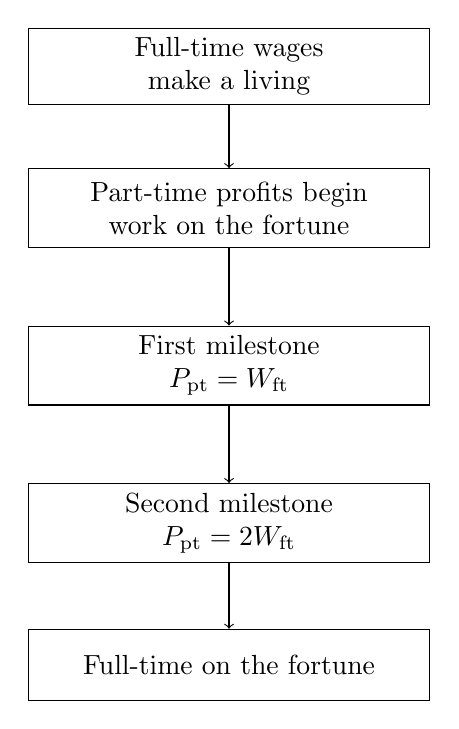
\begin{tikzpicture}
\node[draw, rectangle, align=center, minimum width=5.1cm, minimum height=0.9cm] (a) at (0,0) {Full-time wages\\make a living};
\node[draw, rectangle, align=center, minimum width=5.1cm, minimum height=1.0cm] (b) at (0,-1.8) {Part-time profits begin\\work on the fortune};
\node[draw, rectangle, align=center, minimum width=5.1cm, minimum height=1.0cm] (c) at (0,-3.8) {First milestone\\\(P_{\mathrm{pt}}=W_{\mathrm{ft}}\)};
\node[draw, rectangle, align=center, minimum width=5.1cm, minimum height=1.0cm] (d) at (0,-5.8) {Second milestone\\\(P_{\mathrm{pt}}=2W_{\mathrm{ft}}\)};
\node[draw, rectangle, align=center, minimum width=5.1cm, minimum height=0.9cm] (e) at (0,-7.6) {Full-time on the fortune};
\draw[->] (a) -- (b);
\draw[->] (b) -- (c);
\draw[->] (c) -- (d);
\draw[->] (d) -- (e);
\end{tikzpicture}
\caption{Transcript-derived reconstruction of the lecture's ``magic of part time'' ladder.}
\end{figure}

The lecture then introduces one numerical threshold, not as a theorem but as a social fact. An extra thousand dollars a month is enough, he says, to change the lifestyle of most families visibly.

\begin{equation}
\Delta I \approx \$1000 \text{ per month.}
\end{equation}

The lecture's point is subtle. A thousand dollars a month full time may not attract much attention. A thousand dollars a month part time is different, because it changes what the family can do, and therefore changes what others can see.

\subsection{Question \& Answer}

The lecture naturally raises a question here: why is part-time profit a stronger invitation than ordinary full-time income?

The answer is that the relevant variable is not money in the abstract, but visible change in life. Part-time profit creates a sharp contrast between old circumstances and new freedom. Vacations appear. Cars appear. Clothing appears. The spoken lecture keeps repeating that the real attraction is not merely the cash amount but the lifestyle transformation that cash now makes possible. In note form, the logic is:
\[
\text{part-time profit} \longrightarrow \text{visible lifestyle change} \longrightarrow \text{credible invitation}.
\]

\section{Wind, Sail, and the Possibility of Change}

From the money model Rohn pivots to a more general one. He says that what determines the future is not what happens, but what we do about what happens. The sailboat image is his way of giving this claim operational form.

\begin{equation}
\text{It is not what happens that determines your future; it is what you do about what happens.}
\end{equation}

\begin{equation}
\text{The same wind blows on us all.}
\end{equation}

\begin{equation}
\text{The difference in arrival is not the blowing of the wind but the set of the sail.}
\end{equation}

The transcript occasionally garbles \emph{sail} as \emph{sale}, but the intended image is plainly nautical. The note-writer's compact version is

\begin{equation}
A = A(S;W),
\end{equation}

where \(W\) is the common wind, \(S\) is the sail-setting, and \(A\) is arrival. The point is not a detailed mechanics model. It is a discipline of attention. If the wind is common, then explanation cannot stop with the wind. It must move to what is adjustable.

This is why the lecture immediately shifts into historical and seasonal constants. The next ten years will be about like the last ten. After fall comes winter; after day comes night; after expansion comes recession; after recession comes expansion. Rohn's summary phrase is compact enough to function almost like a theorem of social weather:

\begin{equation}
\text{Opportunity mixed with difficulty.}
\end{equation}

Once that mix is taken as stable, a second law becomes possible.

\begin{equation}
\text{For things to change, you have to change.}
\end{equation}

The transcript is noisy for a few lines in this neighborhood, but the stable pairings are clear from repetition: do not wish for fewer problems; wish for more skill. Do not wish for less challenge; wish for more wisdom. The change variable is personal discipline, not a reordering of the world.

\begin{figure}[h]
\centering
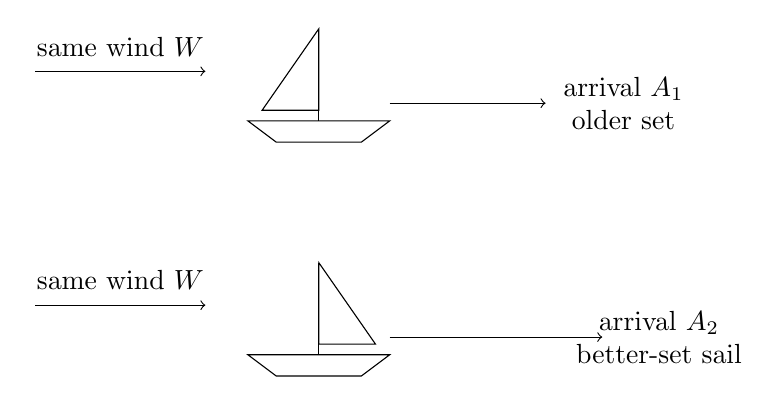
\begin{tikzpicture}[scale=0.9]
\draw[->] (-4.2,1.9) -- (-1.8,1.9);
\node at (-3.0,2.25) {same wind \(W\)};

\draw (-1.2,1.2) -- (0.8,1.2) -- (0.4,0.9) -- (-0.8,0.9) -- cycle;
\draw (-0.2,1.2) -- (-0.2,2.5);
\draw (-0.2,2.5) -- (-1.0,1.35) -- (-0.2,1.35) -- cycle;
\draw[->] (0.8,1.45) -- (3.0,1.45);
\node[align=center] at (4.1,1.45) {arrival \(A_1\)\\older set};

\draw[->] (-4.2,-1.4) -- (-1.8,-1.4);
\node at (-3.0,-1.05) {same wind \(W\)};

\draw (-1.2,-2.1) -- (0.8,-2.1) -- (0.4,-2.4) -- (-0.8,-2.4) -- cycle;
\draw (-0.2,-2.1) -- (-0.2,-0.8);
\draw (-0.2,-0.8) -- (0.6,-1.95) -- (-0.2,-1.95) -- cycle;
\draw[->] (0.8,-1.85) -- (3.8,-1.85);
\node[align=center] at (4.6,-1.85) {arrival \(A_2\)\\better-set sail};
\end{tikzpicture}
\caption{Transcript-derived schematic: the same wind blows on both boats, but different sail-setting produces different arrival.}
\end{figure}

\subsection{Question \& Answer}

If the world keeps sending the same wind, how can a life change drastically?

The answer is that drastic change does not require a new world. It requires a new setting of the sail. Rohn's own example is the simplest possible one: the first six years of his economic life ended in being broke; the second six years ended in being rich. He explicitly rejects the explanation that politics changed on his behalf. What changed, he says, was philosophy, that is, the disciplined form of interpretation and action.

\section{The Law of Averages as Operational Mathematics}

Once agency is established, the lecture introduces its first explicit quantitative law. If we do something often enough, a ratio appears. Once that ratio appears, it tends to continue. In note form, this is the law of averages.

\begin{equation}
R = \frac{s}{n},
\end{equation}

with \(n\) the number of conversations or attempts, and \(s\) the number of affirmative outcomes. Rohn's beginner case is

\begin{equation}
R=\frac{1}{10}.
\end{equation}

Talk to ten people; get one. The importance of this example is not statistical subtlety. It is emotional stabilization. A novice often thinks that a weak ratio means the game is closed. Rohn argues the opposite. Once the ratio is known, planning becomes possible.

\paragraph{Worked example.}
The lecture's competition example is explicit. Suppose an experienced person closes at nine out of ten, while a beginner closes at only one out of ten. Then over a thirty-day contest we may compute

\begin{align}
\frac{9}{10}\cdot 10 &= 9, \\
\frac{1}{10}\cdot 100 &= 10.
\end{align}

The beginner wins, not by superior skill, but by superior volume. The spoken slogan is exact enough to keep:

\begin{equation}
\text{Make up in numbers what I lack in skill.}
\end{equation}

This is the lecture's first real derivation. Skill enters through the ratio; ambition enters through the sample size.

\subsection{Question \& Answer}

How can someone who gets only one out of ten compete with someone who gets nine out of ten?

Because the contest is not ratio alone. It is ratio multiplied by effort. The lecture's answer is not to deny difference in skill, but to offset it by larger \(n\). This is a very characteristic Rohn move. He does not rescue the beginner by saying the beginner is secretly already excellent. He rescues the beginner by showing that arithmetic creates a route for the beginner to stay in the game.

The law then acquires a second feature: it can improve. Repetition does not only reveal a ratio; repetition can change it.

\begin{equation}
\frac{1}{10} \longrightarrow \frac{2}{10} \longrightarrow \frac{3}{10}.
\end{equation}

Why does the fourth round produce two instead of one? Because, as Rohn says, we are getting better. This leads to the baseball analogy:

\begin{equation}
0.300 = \frac{3}{10}.
\end{equation}

Bat three hundred in baseball, fail seven times out of ten, and one is still elite. The operational conclusion is therefore worth writing exactly as he says it:

\begin{equation}
\text{You do not have to bat a thousand to make big money.}
\end{equation}

One out of ten is workable. Two out of ten is strong. Three out of ten is already enough, in the lecture's language, to make one rich beyond prior expectation. This is why he can invite friends to come and ``be one of the seven.'' The arithmetic has already removed panic from the conversation.

\section{Sowing, Reaping, and the Structure of Loss}

The lecture does not stop with ratios, because a clean ratio can still leave us naive about disappointment. Rohn therefore turns to the parable of the sower. Its role in the lecture is mathematical in a broad sense: it converts disappointment from a personal mystery into a structured sequence of loss channels.

The initial conditions are favorable. The sower is ambitious. The seed is excellent. The seed may mean product, opportunity, or story. What follows is not a denial of excellence, but a map of what excellence must pass through.

\begin{equation}
\text{The birds are going to get some of the seed.}
\end{equation}

The first loss channel is pre-engagement theft. Someone intended to come, but did not. In the lecture's folk language, the birds got it. The wrong response is to chase birds. Chasing birds means leaving the field.

\begin{equation}
\text{The hot weather is going to get some.}
\end{equation}

The second loss channel is early withering. Some people begin, grow briefly, then disappear at the first heat. The lecture insists that this is not a puzzle to be psychologized endlessly. Some do not stay.

\begin{equation}
\text{The thorns are going to get some.}
\end{equation}

The third loss channel is distraction. Little cares, little interruptions, small repairs, trash in the garage, ordinary life. The thorns are not dramatic villains; they are precisely the small things that cheat people out of large opportunities.

The lecture then gives its practical moral in one of its strongest lines:

\begin{equation}
\text{You must learn to discipline your disappointment.}
\end{equation}

That sentence matters because it keeps two cases separate. If we made gross mistakes, then correction is our responsibility. But if loss occurs in the normal structure of the thing, then the right response is neither rage nor endless ``why?'' inquiry. The right response is to keep sowing.

\begin{figure}[h]
\centering
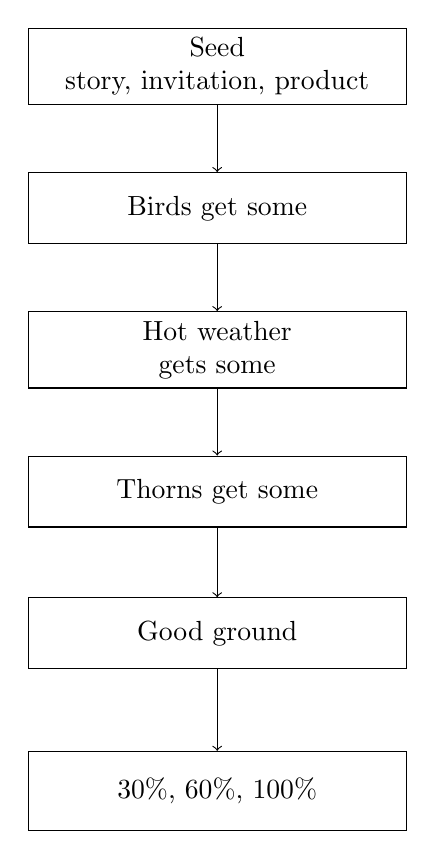
\begin{tikzpicture}
\node[draw, rectangle, align=center, minimum width=4.8cm, minimum height=0.9cm] (s) at (0,0) {Seed\\story, invitation, product};
\node[draw, rectangle, align=center, minimum width=4.8cm, minimum height=0.9cm] (b) at (0,-1.8) {Birds get some};
\node[draw, rectangle, align=center, minimum width=4.8cm, minimum height=0.9cm] (h) at (0,-3.6) {Hot weather\\gets some};
\node[draw, rectangle, align=center, minimum width=4.8cm, minimum height=0.9cm] (t) at (0,-5.4) {Thorns get some};
\node[draw, rectangle, align=center, minimum width=4.8cm, minimum height=0.9cm] (g) at (0,-7.2) {Good ground};
\node[draw, rectangle, align=center, minimum width=4.8cm, minimum height=1.0cm] (o) at (0,-9.2) {\(30\%\), \(60\%\), \(100\%\)};
\draw[->] (s) -- (b);
\draw[->] (b) -- (h);
\draw[->] (h) -- (t);
\draw[->] (t) -- (g);
\draw[->] (g) -- (o);
\end{tikzpicture}
\caption{Transcript-derived reconstruction of the sower story as a vertical filter model.}
\end{figure}

In compact note form we may summarize the model as

\begin{equation}
\text{Seed} \longrightarrow \text{loss channels} \longrightarrow \text{good ground} \longrightarrow \{30\%,60\%,100\%\}.
\end{equation}

The final feature is especially important. Good ground is not uniform. Some outcomes are \(30\%\), some \(60\%\), some \(100\%\). Rohn explicitly warns against a managerial fantasy in which we force every \(30\) into a \(60\). Let the thirties do thirty, the sixties do sixty, the hundreds do one hundred. The aim is not uniformity, but durable movement.

\subsection{Question \& Answer}

What do we do when some do not come, some do not stay, and some are choked off by small distractions?

We do not chase birds, and we do not register for the ``why is it like this?'' class. Instead we cooperate with the structure of the field. The law of averages told us that repetition produces a ratio. The sower story tells us why repetition is morally difficult: losses are real, repeated, and partly outside our making. The discipline is to continue sowing until the seed falls on good ground, because, as the lecture insists, if we keep sowing, eventually it will.

\section{From Philosophy to Skill: Sales, Recruiting, Organizing, Communication}

Only after the laws of profit, wind, ratio, and sowing are in place does the lecture turn to skill. This order matters. The skills are not a disconnected catalog. They are the implementation layer of the earlier philosophy.

The first skill is sales. Rohn deliberately de-technicalizes it. In this business, sales is not an exercise in engineering complexity. It is representation, sharing, testimony, and persuasion simple enough that the buyer sees value and chooses participation. He remarks that learning sales multiplied his income by five. The exact multiplier should be taken as autobiographical, but the structural point is stable: sales is the first entrepreneurial skill that converts enthusiasm into flow.

The second skill is recruiting, and here the lecture becomes more interesting. Recruiting is not only invitation. It is invitation, presentation, and follow-up. Once a new life begins, it must be nourished like a mother nourishes a child and protected like a father protects one. This is one of the lecture's strongest reconceptualizations. Sponsorship is not clerical assistance; it is bridge work. The sponsor carries a person from darkness to light, from skepticism to faith, from discouragement to confidence.

The third skill is organizing. Once a few people exist, the problem is to get them to work together. Rohn treats this as both difficult and magical. The power of shared testimonials is his concrete example. A new person's decision may turn less on my own testimony than on the testimony of someone working beside me. Thus organization magnifies credibility.

Promotion follows. The lecture makes a subtle distinction here: the company creates major promotions, but the local leader must create smaller ones. Small recognitions for small steps become a way of moving people to act beyond what they would ordinarily do alone. That is why promotion, in Rohn's account, pays ``staggering money.'' It is not mainly the money that works magic, but ingenuity.

Communication then appears as the repeated act of doing it again. The early presentation is uncomfortable; the first attempt is poor; one may step out from behind the podium and not know how to get back. Yet the law of skill acquisition here is brutally simple. He did it again. Then again. Then again. In the lecture's rhythm, this is the spoken analogue of the ratio law. Repetition is not merely toleration of embarrassment. It is the process by which embarrassment becomes fluency.

Finally, training, teaching, and inspiring widen the scope. Training is how the business works. Teaching is how life works. Inspiration is the gift of helping people see themselves better than they are, and more capable in the future than they are in the present. The speaker's own mentor did this for him, and that is why the lecture repeatedly ties technical growth to a prior act of imaginative recognition.

\section{Service, Greatness, and the Good Life}

The recruiting section naturally opens into a larger question: what is the underlying law of greatness? Rohn attributes the answer first to biblical teaching, then restates it through John Kennedy and Zig Ziglar. Greatness, fortune, and influence arise by service to many.

\subsection{Question \& Answer}

How do greatness and fortune actually arise?

Rohn's answer is not inward withdrawal and not mere self-protection. It is service outward. In compact note form we may write

\begin{equation}
\text{Service to many leads to greatness.}
\end{equation}

and, schematically,

\begin{equation}
Y \uparrow \qquad \text{as} \qquad N_{\mathrm{served}} \uparrow,
\end{equation}

where \(N_{\mathrm{served}}\) is the number of people directly and indirectly affected, and \(Y\) stands for pay, influence, or recognized greatness. The lecture does not give a formal function. It only insists on the monotone direction. If one affects a few lives, one is paid accordingly; if one affects many, one is paid accordingly.

This same law is stated in two memorable reformulations. Kennedy's version is ``don't ask'' what the people can do for you; ask what you can do for the people. Ziglar's version is:

\begin{equation}
\text{If you help enough people get what they want, you can have everything you want.}
\end{equation}

The late part of the lecture then adds a second organizing rule: respond to deserve, not to need. The sower already implied this. Harvest follows planting, not mere need. The sponsor's practical version is a response rule:

\begin{equation}
1 \mapsto 2,\qquad 2 \mapsto 5,\qquad 0 \mapsto 0.
\end{equation}

That is, one step from the other person earns two from us; two steps earn five; no step earns no step. This is not a theorem of ethics. It is a practical rule for allocating time. It is how one teaches people to deserve attention.

The lecture then adds the well-known imbalance

\begin{equation}
80\% \text{ of the people do } 20\% \text{ of the business.}
\end{equation}

The conclusion is managerial rather than metaphysical: work with a small share individually and the majority by group. Group work is less confrontational, and it is also necessary because there is a limit to carrying.

\begin{equation}
\text{You can help a thousand, but you can't carry three on your back.}
\end{equation}

The companion principle is equally sharp:

\begin{equation}
\text{You cannot change people, but they can change themselves.}
\end{equation}

The pear tree remains a pear tree. Apples hung on it do not alter its nature. This is one of the places where the lecture protects the ambitious organizer from missionary exhaustion. We may help, teach, sponsor, invite, and respond. We may not substitute ourselves for the other's act of change.

The speaker then briefly restates the entrepreneurial rule of sequence:

\begin{equation}
\text{You can either buy and sell, or sell and buy.}
\end{equation}

The point is not accounting technique but initiative. Ambition can begin before capital is abundant. In the lecture's language, even a dollar and some ambition may be enough, and in some cases not even the dollar is first. The story itself can sell, and selling can precede buying.

The closing movement turns away from business mechanics toward life architecture. The greatest value is not the bank account but the good life. The lecture's short list is productivity, good friends, spirituality, attention to words and culture, the inner circle, and finally participation in what he calls the miracle process. The final economic sentence of this whole widening movement is worth preserving, because it ties life quality back to earning power without reducing life to earning:

\begin{equation}
\text{If you live well, you will earn well.}
\end{equation}

The point is not mystical. A life well lived shows in voice, face, magnetism, and presence. Thus the lecture ends not by abandoning its practical concerns, but by embedding them inside a thicker account of nourishment, love, friendship, and disciplined attention.

\section{Summary}

The lecture's structure is unusually coherent. It begins with autobiography but uses autobiography only to launch a sequence of laws. First comes the economic asymmetry between wages and profits. Then comes the part-time ladder. Then comes the sailboat model of change: common wind, adjustable sail. Then comes the law of averages, where ratios turn effort into a computable strategy. Then comes the sower, where disappointment is redescribed as structured loss. Only after these layers are in place do the skills of sales, recruiting, organizing, promotion, communication, teaching, and inspiration appear as the concrete means of action.

The final widening is equally deliberate. Service to many becomes the route to greatness; deserving replaces mere needing as the criterion of response; the good life becomes the environment in which all these disciplines are to be housed. The lecture's ceremonial ending should therefore be taken seriously. The notes are not merely a record of what was said. They are the device by which the lecture continues after the room goes dark.